\chapter{Topic Modeling}

In Chapter \ref{wordemb}, we presented some techniques to encode words as vectors.
Starting from a bag-of-words model in which we assume that the order of the words
inside a text does not matter, it is possible to follow a similar approach also for documents.
Topic models play an important role in describing, organizing and comparing unstructured collections of documents.

The first step is to generate a matrix of term counts $X$ for the entire corpus:
each row is a document represented in the BOW format and each column represents the count of occurrence
of a particular term in the documents.

The goal of the second step is to produce two matrices:
\begin{itemize}
    \item term-topic matrix: each row represents how related each term is to all topics
    \item document-topic matrix: each row represents how related each document is to all topics
\end{itemize}

For instance, a document about bears is likely to have high intensity on some topics which in turn have high
intensity on words related to animals; see Figure \ref{fig:topicmat} for an example.

\section{Latent Semantic Analysis (LSA)}
Given the number of topics $V$ as an hyperparameter,
Truncated SVD is applied to the matrix obtained in the first step
(see Figure \ref{fig:svd} for a graphical representation):
$$X_{N \times K} = U_{N \times V} \Sigma_{V \times V} D_{K \times V}^T$$

The matrix $U$ is then used as the document-topic matrix,
while $D$ represents the term-topic matrix.

Using $U$ instead of $X$ for comparing documents when $V \ll K$ leads to a smaller memory footprint.
Furthermore, the terms are no longer orthogonal: thanks to this it is possible to compute the similarity between
a term and a document even if the document does not contain the term itself.
The key point to observe is that both terms and documents are described as topics: if a term is frequent in some topics and
a document is frequent in the same topics, they will have a similar representation in the new space.

An overview of this technique can be found at \cite{doi:10.1002/aris.1440380105}.

\begin{figure}[h]
    \centering
    \subfigure{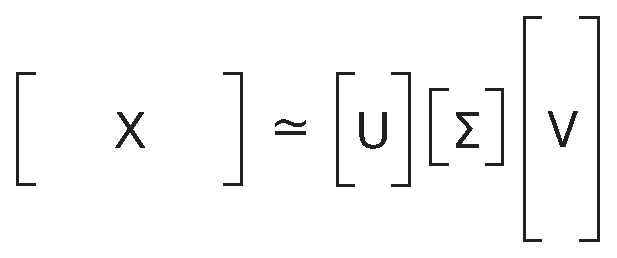
\includegraphics[width=0.5\textwidth]{images/svd.eps}}
    \caption{Truncated SVD represented graphically; matrices size proportions are kept intact}
    \label{fig:svd}
\end{figure}

\begin{figure}[h]
    \centering
    \subfigure{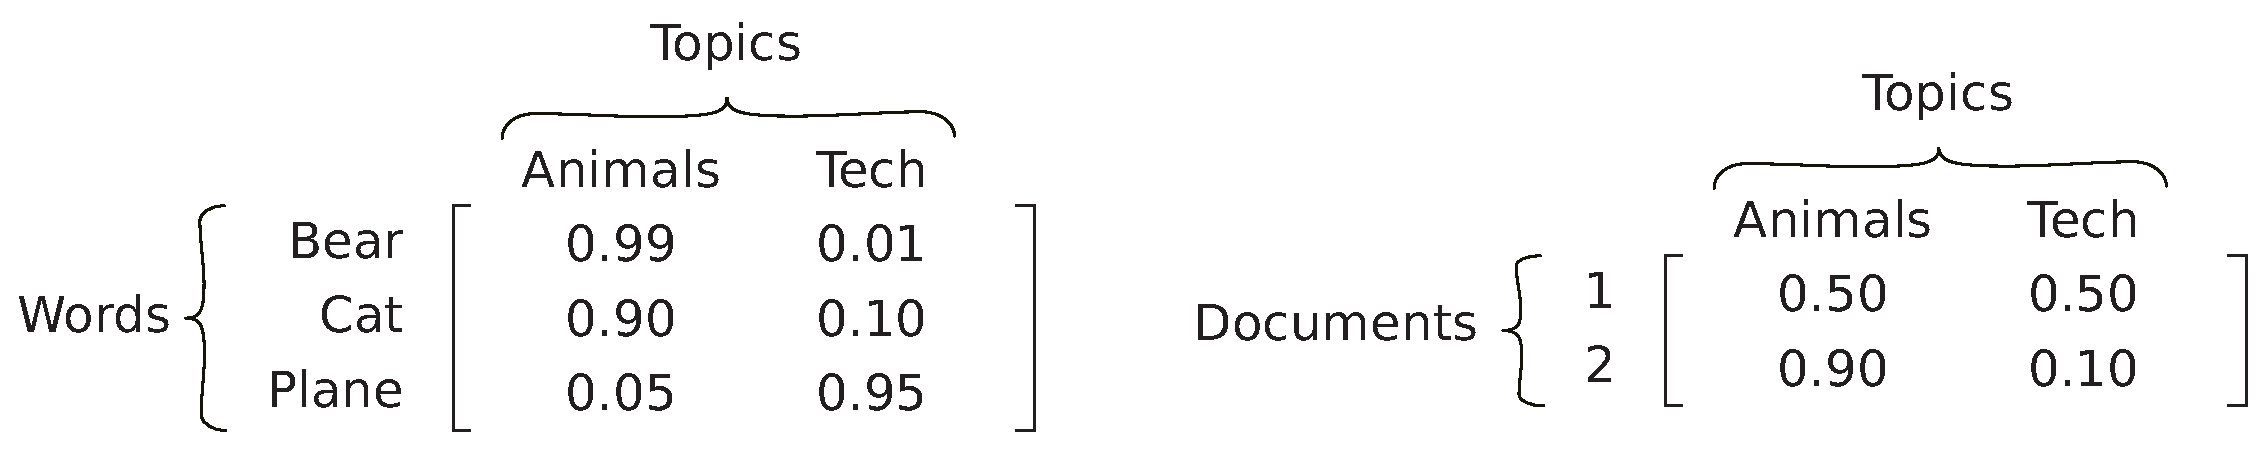
\includegraphics[width=\textwidth]{images/topic-mat.eps}}
    \caption{Example of a term-topic and a document-topic matrix.}
    \label{fig:topicmat}
\end{figure}

\section{Latent Dirichlet Allocation (LDA)}
LDA makes the same assumptions about topics as LSA, but unlike the latter it views topics and documents in a probabilistic way.
In particular, a document is a categorical distribution over topics $\theta_d$ and a topic is categorical distribution over words $\beta_i$.
The probability of sampling a particular document is instead modeled as a dirichlet distribution $Dir(\alpha)$.

A major drawback of LDA is that the number of topics is assumed to be known a-priori and threated as an hyperparameter.

Variants of this model are present in the literature: in this chapter we use \cite{10.1145/2107736.2107741} and \cite{DBLP:journals/jmlr/BleiNJ03} as a reference.

\subsection{Generative process} \label{gp}
In this section we describe LDA by its generative process, assuming we have already obtained the parameters of the model.

We define:
\begin{itemize}
    \item $\beta_{1:K}$: $K$ topics, where each topic $\beta_i$ is a distribution over the terms in the vocabulary
    \item $\theta_d$: a document $d$ described as a categorical distribution over topics, where $\theta_{d,k}$ is the topic proportion for topic $k$ in document $d$
    \item $w_{d}$: observed words of document $d$, where $w_{d,n}$ is the word in position $n$ of the document $d$
\end{itemize}

The generation of $M$ documents with $N$ words each can be summarized as:
\begin{enumerate}
    \item $\theta_d \sim Dir(\alpha)$: pick a document
    \item $z_{d,n} \sim Mult(\theta_d)$: sample a topic
    \item $w_{d,n} \sim \beta_{z_{d,n}}$: pick a term
    \item use that term as a word for the document you want to generate
    \item loop $N$ times to step 2
    \item loop $M$ times to step 1
\end{enumerate}

LDA can be seen as a probabilistic graphical model and it is represented graphically in Figure \ref{fig:lda}.

The joint distribution is:
\begin{equation*}
    \begin{split}
        p(\theta, z, w | \alpha, \beta) & = \prod_d p_d(\theta, z, w | \alpha, \beta) \\
        & = \prod_d [p(\theta_d | \alpha) \prod_n p(z_{d,n} | \theta_d) p(w_{d, n} | \beta, z_{d,n})]
    \end{split}
\end{equation*}

Given the distributions explained before, we can state that:
$$ p(\theta_d | \alpha) = \frac{1}{B(\alpha)} \prod_{k=1}^K \theta_{d,k}^{\alpha_k - 1}$$
$$ p(z_{d,n} | \theta_d) = \theta_{d, z_{d,n}} $$
$$ p(w_{d,n} | z_{d,n}, \beta) = \beta_{z_{d,n},w_{d,n}} $$

\begin{figure}[h]
    \centering
    \subfigure{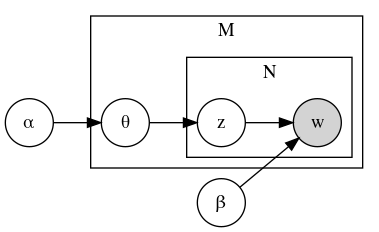
\includegraphics[height=150px]{images/lda.png}}
    \subfigure{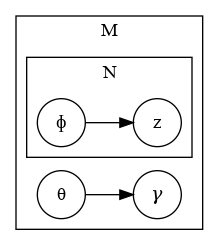
\includegraphics[height=150px]{images/lda-vi.png}}
    \caption{Graphical model representation of LDA (left) and graphical model representation of the variational distribution (right). Nodes are random variables, shaded if observed. An edge denotes a possible dependence between random variables. Plates denotes multiplicity.}
    \label{fig:lda}
\end{figure}

\subsection{Model inference}
The goal of LDA is to automatically discover topics over a collection of documents.
Since only words are observed, topics are considered latent variables.

Note that inference in this particular case can be seen as the reverse of the generative process explained in \ref{gp}.

Mathematically speaking, inference becomes a question of computing the posterior distribution:
$$ p(\theta, z | w, \alpha, \beta) = \frac{p(\theta, z, w | \alpha, \beta)}{p(w| \alpha, \beta)}$$
which is the conditional distribution of the hidden variables given the documents.

The denominator $p(w_{1:D} | \alpha, \beta)$ is the probability of observing the corpus under all possible topic model combinations
and thus intractable to compute.
For this reason in this section we approximate the posterior distribution through a variational method
(see Appendix \ref{vi}).
In particular, we set $q$ as:
\begin{equation*}
    \begin{split}
        q(\theta, z | \gamma, \phi) & = \prod_d q_d(\theta, z | \gamma, \phi) \\
        & = \prod_d q_d(\theta | \gamma) q_d(z | \phi) \\
        & = \prod_d [q(\theta_d | \gamma_d) \prod_n q(z_{d,n} | \phi_{d,n})]
    \end{split}
\end{equation*}
Its graphical representation can be seen in Figure \ref{fig:lda}.

To do model inference from a collection of documents, we start defining the ELBO function:
\begin{equation*}
    \sum_d log_2 [p_d(w | \alpha, \beta)] \geq \sum_d \E_{q_d} log_2[p_d(w, \theta, z | \alpha, \beta)] - \E_{q_d} log_2[q_d(\theta, z | \gamma, \phi)]
\end{equation*}

Since constrained maximization and
the Newton-Raphson algorithm are required to solve the problem
instead of traditional variational inference,
we intentionally present only an hasty description of the update algorithm:
\begin{enumerate}
    \item Initialize $\beta$ randomly, set each $\phi_{d,n}$ as $\frac{1}{K}$ and each $\gamma_d$ as $\alpha_d + \frac{N}{K}$
    \item For each document, update the local latent variables $\gamma$ and $\phi$ until convergence
    \item Update the global latent variables $\beta$ and $\alpha$ for the entire corpus until convergence
    \item Loop to 2 until convergence
    \item The expectation of a given $\gamma$ for a particular document is its topic distribution
\end{enumerate}
Note that the step 2 can be parallelized: each document has its own local variables which are conditionally indipendent
of the other local variables and data in different documents.

The interested reader can find more details looking at Appendix A of \cite{DBLP:journals/jmlr/BleiNJ03}.

\subsection{Sparsity considerations}
Using the dirichlet governed by the $\alpha$ parameter to induce sparsity
allows us to have documents described by fewer topics than using an uninformative prior.
The same reasoning can be applied to topics, introducting a dirichlet that governs the
probability of having a topic with a particular set of terms.

Inducing sparsity combined with a number of topics much less than the number of documents
lower the risk of obtaining two different topics with a similar distribution of words.


\section{Online LDA}
A major drawback of LDA is the impossibility to scale as the data grows:
each iteration of the algorithm requires an entire scan of the corpus, which is computationally expensive.

\section{Hierarchical Dirichlet Process (HDP)}
HDA was proposed in \cite{DBLP:journals/jmlr/WangPB11} to overcome the problem of choosing the number of topics in LDA and derived methods.
In particular this number is not an hyperparameter of the model, but it is determined during inference.
